\documentclass[conference]{IEEEtran}

\usepackage{graphicx}

\usepackage{placeins}

\graphicspath{{Figures/}}



\begin{document}

	\title{A Survey of Range-Only SLAM Techniques and Sensors}
	
	
	
	\author{David Grabowsky, Samyak Shetty, Sam Shue, James M. Conrad}
	
	
	
	\markboth{IEEE Transactions On xxxl, Vol. XX, No. Y, Month 2018}{Grabowsky: RO SLAM}
	
	
	
	
	
	
	
	\maketitle
	
	
	
	
	
	\begin{abstract}
		
		
		
		
A common aspect in many autonomous robotics applications is addressing the problem of Simultaneous Localization and Mapping (SLAM). In most SLAM applications, the robot identifies distinguishable features in the environment, known as landmarks, within the environment through sensors such as cameras and laser rangefinders. Sensing these landmarks provide the robot with information such as range and bearing, which are used in the estimation proses of the robot's pose and the landmark locations within the map. However, some applications use landmarks which are only capable of providing range information, such as wireless and acoutstic beacons. In this survey, the variety of techniques used to solve the SLAM problem with respect to range only sensors (RO-SLAM) is explored.
		
		
	\end{abstract}
	
	
	
	
	
	
	
	\section{Introduction} 
		The Simultaneous Localization and Mapping (SLAM) problem is a common aspect of many autonomous robotics applications. SLAM involves estimating the pose of a mobile robot and building a map of its environment with no a priori information. The SLAM problem is a chicken-and-egg type problem, where the pose of the robot is with respect to a global frame, or map, and building a map requires knowledge of the robot's location. There are many algorithms used to solve this problem, most using a landmark-based approach. The concept of a landmark is identifying a distinguishable feature in the environment through camera or laser rangefinder and estimating the distance and orientation of that landmark relative to the robot. Then, as the robot traverses the environment, it can continue observing that landmark, as well as collecting new landmarks, and using the sensed distances and angles combined with odometry readings to refine its estimation of the robot's pose and map. In most SLAM applications, references to the map is synonymous with the locations of the landmarks.
	
	In outdoor SLAM applications, such as self-driving cars and autonomous farming equipment, global positioning satellite (GPS) readings are used in addition to the vehicle's odometry. While GPS has low resolution, it proves useful as it provides location information, which can help compensate for the accumulated error from drift in odometric sensors. However, GPS isn't available in all environments, such as indoors and underwater. Instead, wireless signals and sonar beacons are often used in indoors and underwater environments, respectively. While these beacons provide sensor information to the robotic vehicle, they don't inherently provide location information unless their positions are accurately known beforehand and are certain to never change. Wireless and sonar beacons are capable of providing range measurements instead.
	
	\section{range only sensors/tech}
	
	One of the key features of the systematic localization and mapping problem are landmarks. In RO SLAM the only information that can be obtained from landmarks is range data. This range data must then be interpreted by the robot in some way that will be advantageous towards the localization and mapping process. Beacons are a popular implementation of landmarks. Beacons refer to any devices which involves a signal transmission that can be used for the localization and mapping process without line of sight. The most popular beacons can largely be broken down into two categories: acoustic based and radio frequency based.
	
	\subsection{Acoustic}
	
	Acoustic ranging systems are primary used with robotics and beacons that operate in underwater locations. The reason for this that radio waves experience strong attenuations, especially in salt water environments. As \cite{Partan2007} states, the issue of attenuations makes radio waves extremely impractical, thus making acoustics the logical alternative. Acoustic still suffer from a range of problems such as multipathing and propagation delays, but are one of the only meaningful alternatives. Papers such as those by \cite{Erol-Kantarci2011} and \cite{Akyildiz2005} explore a wide variety of issue and possible techniques that relate to acoustic sensors, such as the added complexity of assuming a 2D environment vs a 3D environment, or design challenge that accompany underwater deployment like spatial correlation and power. 
  	
	An interesting beacon for underwater localization that is not specifically range only or acoustic based is the Dive'N'Rise (DNR) beacons presented by \cite{Erol2007}. These DNR beacons rise to the surface, receive their location through GPS, then sink into the water and transmit their coordinates. The distance to an agent and the transmitting beacon can be determined via time of flight from the transmissions. A localization implementation using these beacons was accomplished by \cite{Erol2008}. Again while this is not purely range only or acoustic based it was found to be interesting solution worth mentioning.
	
  	\begin{figure}[h!]
	
	\centering
	

%	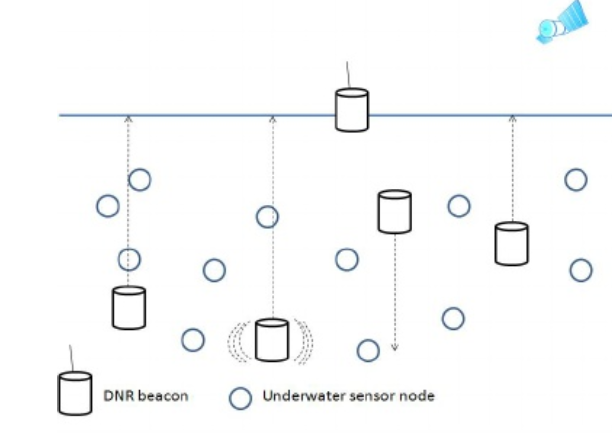
\includegraphics[width=90mm]{DNR.png}

%	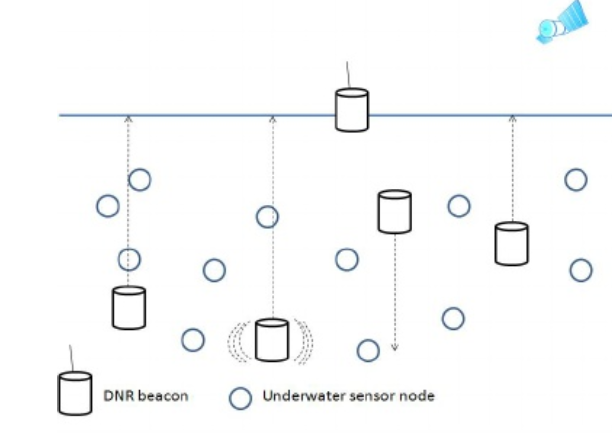
\includegraphics[width=90mm]{DNR.png}
	
	\caption{DNR being used to implement Dive and Rise Localization  \cite{Erol-Kantarci2011}}
	
	\label{DNR}
	
\end{figure}


	\subsection{Radio Frequency}
	Radio frequency encompass a massive spectrum of devices capable of transmitting or receiving transmission on the radio frequency. There are two methods primarily utilized to determine distance from radio frequency. One is by examining the received signal strength indicator (RSSI) and the other is the by measuring the time of flight of the signal. A system presented by \cite{Padmanabhan2000} processes rf signal strength and utilizes nearest neighbors heuristics to achieve localization based on said signal strength.  \cite{Kurth2003a} describes a method for using very small RF tags as beacons throughout the environment.  As a robot moves throughout an environment it emits a query to which any RF tags that are within the transmission range respond to. The robot then estimates the distance to the tag based on the delay. The response from the RF tags include a data tag which contains a unique ID number. 
	
	Wireless sensors networks (WSN) are also a very popular choice, especially since many of them come with the ability to transmit RSSI. \cite{Baronti2007}, \cite{Khanafer2014}, \cite{Akyildiz2002}, and \cite{Xia2011} each presents surveys relating to WSNs.  \cite{Baronti2007} and \cite{Akyildiz2002} both provide very well developed survey that discuss hardware, protocols, standards, security, energy efficiency and much more. \cite{Baronti2007} specifically focuses on state of the art 802.15.4 and ZigBee standards. \cite{Xia2011} examines the limitations of original IEEE 802.15.4 MAC and reviews adaptive methods that have been used to overcome these limitations. \cite{Khanafer2014} specifically survey methods meant to improve the performance of IEEE 802.15.4 MAC protocol.




	%blue tooth
	
	
	%wifi
	
	%Fingerprint map based on radiological patterns
	%P. Bahl and V. Padmanabhan, “Radar: A, in-building rf-based user
	%location and tracking system,” in Proc. of the IEEE Infocom, 2000,
	%pp. 775–784.
	
	%M. Oca ̃na, L. M. Bergasa, M. A. Sotelo, R. F. Flores, D. F.  ́
	%Llorca, and D. Schleicher, “Automatic training method applied to
	a% WiFi+ultrasound POMDP navigation system,” Robotica, vol. 27,
	%no. 07, pp. 1049–1061, December 2009.
	
	
	%rfid
	%Mapping and localization with RFID technology
	
	

	
	


	


\section{Beacon Initialization}
Beacons initialization refers to the process by which beacons (or landmarks) at an unknown position receive their initial position estimation. One of the complications with RO-SLAM involves the issue of determining the location of landmarks when their initial placement is unknown, the EKF, which is used by many implementations, is especially sensitive to poorly initialized landmarks as they are used as the basis for the convergence of an accurate estimate. Poorly approximated landmarks results in the divergence of the filter. These methods are further  divided into delayed and undelayed initializations.
\subsection{Delayed/Offline initializations}
These are methods that perform delayed localizations  where initially the robot moves around offline collects some measurements and then initializes the location of the landmarks. This can be undersirable as it causes a delay in the localization of the robot whenever there is a immediate real time application such as in autonomous vehicles. Localization can be performed only once a accurate estimations of the beacons are made. There are several offline algorithms that perform localization such as the least squares approach in[5 of Active range only beacon lov=calisationi],a posed based ekf as mentioned in[8] , a moving horizon estimation as mentioned in [9] etc. The most popular ones are mentioned below.

\begin{figure}
	\centering
	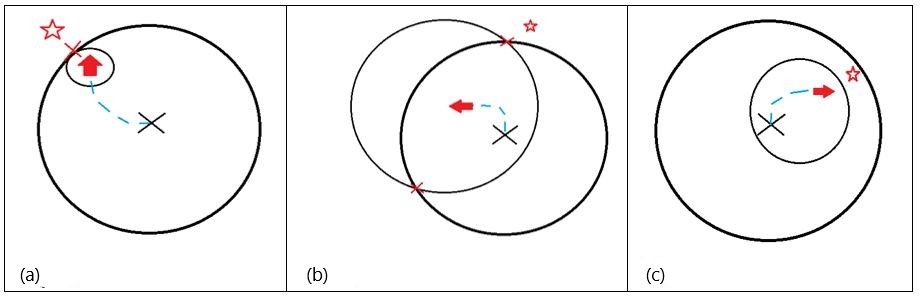
\includegraphics[height=40mm,width=90mm]{Trilateration_methods.JPG}
	\caption{The red arrow represents the robot.The 'X' represents the origin of the robot. The blue line shows the traversed path.The star represents the landmark. }
	
\end{figure}
\subsubsection{Trilateration}
[Pure Porbablisitc approach to RO  SLAM] mentions a basic trilateration technique involving geometric intersection. Rings are drawn at different points of the robots path as shown in Fig[a] , where the radius of the rings depend on the strength of the received signals from the beacons. This method of initialization is highly ambiguous as the rings can have more than 1 point of intersecting as shown in Fig[b]  or no  intersecting points as shown in Fig[c]. %more paperes needed
\subsubsection{Particle filter}
This takes a more probabilistic approach to estimating the initial location of the beacons. As mentioned in[thrun particle filter paper] initially the entire space is represented by particles. These particles are resampled based on importance weights every iteration. There are several resampling methods mentioned in[methods paper]. Eventually the particle set converges to the accurate location of the beacons. Though this method of localization can be computationally expensive it is preferred whenever the noise involved is non Gaussian.

\subsection{Undelayed/Online initializations}
In this case the robot simultaneously initializes and localizes itself and the beacons as it moves
as mentioned in \cite{Caballero2010}. A Gaussian Mixture Model is integrated into the EKF to create a multiple hypothesis filter.  This multiple hypothesis approach is used to solve the RO-SLAM problem and its use allows for the un-delayed initialization of landmarks, however a large number of hypothesis can lead to increased computational burden. \cite{Geneve2015} also puts forward a method that utilizes a Gaussian mixtures for beacon initialization in EKF, but in this method only two hypotheses and a Cartesian plane. \cite{Ahmad2011a} proposes to reduce the computational burden of methods, such as the one proposed by \cite{Caballero2010}, by introducing a novel state vector that eliminates the need for multiple hypothesis landmark representation. The paper proposes that under different circumstances the landmark could be represented using different parameters. Four circumstances are presented in the paper and the method is tested in simulation using both the EKF and a least squares optimization approach. The results showed that when the circumstances can be clearly distinguished between, an increase in performance is seen.



	
	

	\section{Methods and Their Implementations}
	
	\subsection{EKF}
	
	%breif description (1-2 paragraphs)
	
	%paragraphs 
	
	The Extended Kalman Filter (EKF) is one of the most popular and widespread methods used to solve the SLAM problem. It is used to overcome the assumption of linear state transitions and measurements, which are rarely seen in practical environments \cite{Thrun2002}. The derivation of the EKF is very well documented, as such, detailed explanations can be viewed from a variety of sources such as: \cite{Thrun2002}, \cite{Ribeiro2004}, and \cite{Haykin2001}. When used to solve SLAM the map applied to the EKF is a feature based map, meaning it is composed of observable features (landmarks) which can be distinguished between during re-observation \cite{Thrun2002}. This distinction becomes important when examining range only SLAM (RO-SLAM) where only the range to a landmark, or the range between landmarks, is known. This restriction means that landmarks often need to be manufactured, such as the beacons discussed in previous sections, and physically placed in an environment. However, that does not mean that the exact location of the landmarks, or even there initial existence, is recognized. Initialization is a critical element in many algorithms that make use of the EKF. If the initialization is inaccurate then the convergence to a correct estimation becomes much more difficult for the filter. The EKF has seen a wide variety of implementation ranging from ground based robotics\cite{Djugash2008}, to unmanned air vehicles \cite{Fabresse2016}, and to autonomous underwater vehicles \cite{Olson2006}. This section will proceed to give a summary of the various ways EKF has been implemented in regards to RO SLAM, as well as examine improvements to the general RO SLAM problem that are applied via methods with EKF mind.
	
	
	
	A system for robust range only localization was prosed by \cite{Olson2006}. The system utilized an Autonomous Underwater Vehicle (AUV) and beacons without carefully surveyed locations. The paper notes that one of the majors issue was noise present in the received data. A method for outliers rejection caused by the noise was accomplished via spectral graph partitioning. A voting scheme was implemented similar to a Hugh transform to get approximate beacon locations \cite{Hough1959}. The approximate locations were then incorporated into an EKF. It is noted by the paper that this method is particularly CPU intensive, however they state that since the rate at which data is acquired from a landmark is slow, every 5 or so seconds, that the AUV can afford the expensive computation since there will be an adequate amount of time between readings for the data to process. The methodology was simulated using a dataset and can be seen in the paper.
	
	
	
	\cite{Kurth2003} presents a comparison of how three methods process a collected data set. The methods are a EKF, a sliding batch, and a particle filter. The comparison considers the cross-track error, and along track error. The results state that the particle filter works well when used to acquire an initial pose estimate, and EKF works well with real-time localization. It is suggested that in the future that the two could be switched between when appropriate to improve the overall system. 
	
	
	
	
	
	
	
	%fabreese. 
	
	%1. 2013 presents EKF slam method for ariel vehicles 
	
	%2. 2014 introduces prefiltering to measurments for previous 
	
	%3. 2014a integrates visual landmakrs as well
	
	%4  2015 decentralized multiple arieal vehicles
	
	%5  2016 specifically unmaned ariel, more details on 2013,2014 and experimental validation of 2013,2014.
	
	
	
	\cite{Vallicrosa2015} presents a solution utilizing a Sum of Gaussian (SOG) filter for a single range only beacon. It uses multivariate Gaussian mixtures to represent the probability distribution functions of the robot and beacon positions as Gaussian particles which each contain an EKF for vehicle position, velocity, and estimated beacon position. The paper presented experimentation where the method was used to map a beacon while correcting the navigation of the vehicle. 
	
	
	
	Several techniques have also been implemented that involve cooperative sensors. Traditionally sensors were used to only determine the range between themselves and the robot. The sensors in these cases provide the ability determine the range between themselves and other sensors and or the robot \cite{Patwari2005}.
	
	\begin{figure}[h!]
		
		\centering
		
		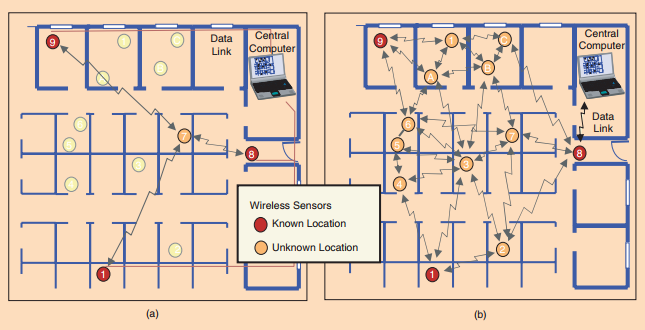
\includegraphics[width=90mm]{coop_loc_comp_patwari.png}
		
		\caption{Traditional(a) vs Cooperative(b) Sensors \cite{Patwari2005}}
		
		\label{trad_vs_coop_sensors}
		
	\end{figure}
	
	\FloatBarrier
	
	
	
	It is explained by \cite{Torres-Gonzalez2015} that methods utilizing inter beacon measurment should incorporate measurements with a configurable number of hops between beacons. This allows for the robot to gather range data from beyond the extent of the robots sensors. Experimentations was conducted utilizing this method via a particle filter EKF. The results showed that the more hops that were added the greater the performance of the system. 
	
	
	
	\cite{Djugash2006} presents a comparison of multiple RO SLAM methods utilized in two scenarios. One scenario involves the case where the robot only has access to range information between itself and beacons at unknown locations. In the second case the robot also has access to information about beacon to beacon distances. Several separate methods were compared in the given scenarios utilizing a data set and experimentation. The first method utilizes the Kalman filter in the case where only measurment between moving and stationary beacons are considered. Another method specifically uses the beacon to beacon measurements with an online Kalman filter. An off line batch method is used to get an estimate of the beacon location and robot path. Finally an method that considers the robot as a virtual node for creating submaps to be solved with a multidimensional scaling algorithm is also considered. The paper gives experimental results and analysis for each of the methods. 
	
	
	
	%In scenarios where the location of the landmarks is unknown and each landmark can not communicate with all every other landmarks, \cite{Djugash2006} presents a solution. He proposes that a moving beacon be used to add edges to the network \cite{Djugash2006}. In addition, no external position sensing were required on the part of the moving beacon, but the option for it to be incorporated was available. 
	
	
	
	
	
	
	An extension to EKF called relative-over parametrized (ROP) EKF is presented by \cite{Djugash2008}. This extension uses specific parameterization to  better represent the range only data utilized in RO-SLAM. ROP EKF operates in polar coordinates as opposed to the Cartesian space that typical EKF operates. The method provided improved results over EKF when sparse range measurement or data association errors were present. \cite{Herranz2014} presents a comparison of the ROP-EKF method presented by \cite{Djugash2008}, to a smoothing and mapping method presented by \cite{Dellaert2006}. Experimentation conducted by \cite{Herranz2014} on and indoor and outdoor environment show an improvement in the results of the SAM method over ROP EKF.
	
	\begin{figure}[h!]
		
		\centering
		
		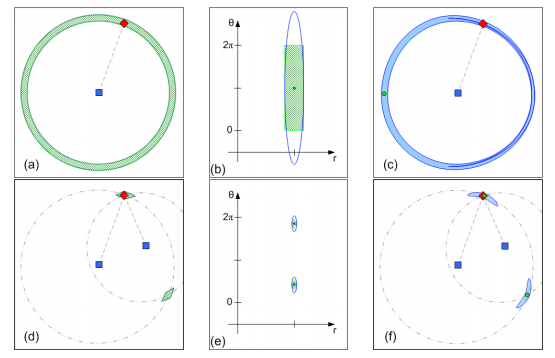
\includegraphics[width=90mm]{ROP_djugash.png}
		
		\caption{Top Row: True and approximated distribution from one range observation. Bottom Row: True and approximated distributions with two observations from different locations. Left Column: Distribution in Cartesian Coordinates. Middle Column: True and Gaussian approximated distributions in Polar Coordinates, Right Column: Projection of the Gaussian approximated. \cite{Djugash2008}} 
		
		\label{ROP_djugash}
		
	\end{figure}
	

	
	
	
	
	
	A method proposed by \cite{Dios2015} is geared towards improving map building speed and accuracy for UAS dealing with the 3D RO-SLAM problem. The 3D RO-SLAM problem refers to the added complexity that devices such as submersibles \cite{Newman} and aerial vehicles experience when having to operate in an environment where three dimensions must be considered as opposed to the planar environment many robots are assumed to operate in. The method utilizes inter-beacon measurements and a novel mode selection which is used to select a measurement gathering method based on current conditions \cite{Dios2015}. The first mode is noted as mapping (MS) and the second localization (LS). When in mapping mode the measurment are integrated with a high probability to quickly create a map, when in localization mode the probability is lowered to create higher accuracy localizations. Based on experimentation performed by \cite{Dios2015} the method performed well and a general increase in accuracy and map speed was noted, however it is stated that a wider variety of experimentation should be performed to validate the overall robustness and effectiveness of the method.
	
	%this one might need some more work
	
	
	
	It is explored by \cite{Kehagias2006} how interpolation can be used to generate range data that is equally spaced over time as opposed to the irregular time intervals that range data is typically received at and then applied to solve the RO SLAM problem. The method is tested on the EKF and an batch optimization algorithm with a simulated and physical robot. The results provided by the paper show that the interpolation based algorithms gave better landmark estimation than those without, with the exception of the EKF in two datasets where EKF was already performing poorly.
	
	
	
	
	
	\cite{Fabresse2013} presents a solution for the 3D RO-SLAM problem. The solution reduces computational load through reduced spherical parametrization of map feature positions. The paper also proposes a new EKF update method which incorporates a reduced spherical representation of the state vector. In addition the paper describes how to efficiently integrate multi-modal belief of elevations angles and azimuth from a range sensor into the EKF utilizing two independent Gaussian Mixtures \cite{Fabresse2013}. In addition \cite{Fabresse2014} expands upon this by presenting a pre-filtering algorithm to be applied to range measurment before being used in the EKF in order to reduce the effect of noise generated by environmental issue such as multipathing. It is then proposed by \cite{Fabresse2015} that the above method can be utilized for decentralized multi-SLAM with range only sensors. This new method would allow for landmarks estimated by a robot to be incorporated into the estimation of another nearby robot, thus improving localization estimation. Based on experimental results obtained by \cite{Fabresse2015} the integration of estimates from multiple robots of the same landmarks provides a benefit to landmark localization over a single robot. In \cite{Fabresse2016} the author also validates and expands upon this method through indoor and outdoor experimentation with an Unmanned Aircraft System (UAS).  
	
\subsection{Sparse Extended Information Filters}
Need to add references

Information filters work on same underlying Gaussian belief principle as that of EKF but vary in the way the Gaussian beliefs are represented. An IF algorithm is mentioned in[ probobilistic robotics book]. In EKF the gaussians are represented in the form of their moments; mean and variance, whereas in a information filter the gausiians in their conical parameterization which is comprised of a information matrix and information vector.Hence what is computational complex in EKF is simple in the other and vice versa. Hence they are dual to each other.
Sparse Extended information filters is derived from the information filter Information filters but it maintains a sparse representation of the information matrix. This makes the SEIF more scalable and effiecient as show in [SEIF paper1] 

The information filter stores the relation between any 2 state elements in the information matrix also known as links. The higer the vlaue of the link the stronger is the relationship between the 2 state variables and the more it is gonna effect the robot s state . SEIF maintains a sparse information matrix by eliminating weak inks that are below a certain threshold thus reducing the computational complexity involved .

In [SEIF PAER 1] they further reduce the computational complexity of by utilizing the computational capabilities of the nodes or radio  beacons. Here the robot computes the preditcition stage of the iteration, send the information to the beacons where they compute the update of the process. Hence the computer burden on the robot is reduced. In addition they factored in inter beacon measurements to reduce uncertainity even furthur. In [seif paper 2] it evaluates and compares  the SEIF method for 3d SLAM using an octorotor In conclusion this menthod had better estimates and lesser computational burden than the traditionl RO SLAM mehtod using EKF. 



	
	
	
	
	\subsection{Graph SLAM}
	
\subsection{Particle}      %change the references
Particles filters are made ue up various monte carlo algorithms. they are used to estimate states in partially observable Markov chains as shown in [9]. In  initial applications particle filters were used in the field of localization where it was used to estimate a robots pose from sensor data. It is considered better and more robust to conventional estimation methods because it was able to solve the global localization[2] and the kidnapped robot problem[14] which EKF in comparison has it drawbacks. It has also been at the core higher dimensional computational problems.  
%Description
Initially robot assumes global uncertainity through a set of particles that are distributed all over the map. Hence both the robot and the landmarks are uncertain.As the robot moves around and measures sensor data it resamples the particle set weighted according to the probability of the particle being the right one. There are several resampling methods depending on computational complexities[sampling methods paper]. After some iterations only the particles which have a high degree of probability  remain and eventually converge to the state of the robot and the landmarks.
\begin{figure}[h!]
	\centering
	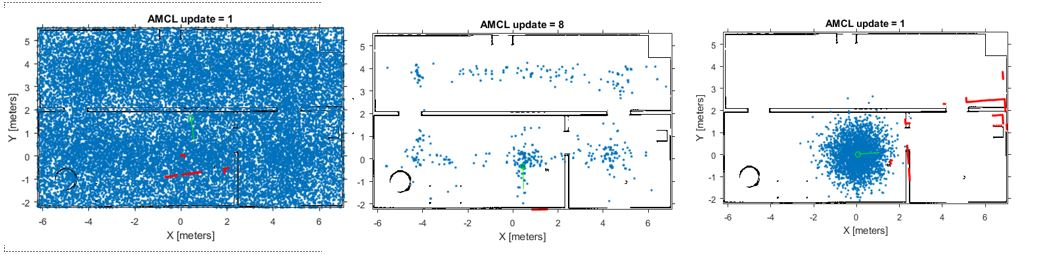
\includegraphics[height=40mm,width=90mm]{Particle_filter_method.JPG}
	\caption{The leftmost image describes the state of the robot when it just initializes the particle filter. The particles are uniformly distributed.The image in the center describes the particle filter after a couple of iterations. Only the particles which have a higher probability are re sampled. The image on the right shows the particle filter eventually converging to estimate the robot location. }
	
\end{figure}
Assuming at time t=0;we have N particles equally space in the enviornment that are drawn based on a uniform distribution $ p(x_oa)$.                                                                        resampling methods depending on computational complexities. After some iterations only th   p
Once the robot starts moving it collects measurements and at time $t>0$ we sample a new particle set $x^{[i]}_t$ for each particle in $x^{[i]}_{(t-1)}$. It is sampled based on the probability of measurement $p(z_t|x^{[i]}_{(t-1)})$. Eventually the particle filter converges to give us the true positioning of the robot.


As mentioned in[thrun particle] particle filters outperform EKF in applications involving global localization (the kidnapped robot problem ) where the robot is randomly picked up and placed in a unknown environment. 
EKF cannot process negative information, but since particle filters use raw sensor data without any processing they can process negative information[probablistic robotics]
As the number of particles increases the computational complexity of the filter too increases. In order to address this there were several new methods introduced that  exploit the independence among state variables. For example the Rao-Blackwellized particle filters that exploit the independence of the landmarks with the robot path thereby reducing the computation complexity from [Fast slam paper]. It also solves the data association problem previously unsolved by EKF[8].
	

	
	\subsection{Fast SLAM}
	EKF is mainly used when we have a non-linear dynamic system model which has Gaussian noise.The quadratic complexity due to Gaussian approximations of higher dimensions make the covariance matrix very large. This eventually causes higher complexity and leads to the divergence of the filter. The single data association problem also adds to this complexity. FastSLAM uses multiple hypothesis data association through particle filtering to overcome this problem. This allows it handle system models with non gaussians noise as well. This results in the computational complexity to grow logarithmically instead of quadratic growth.
	
	FastSLAM utilizes the conditional Independence property of SLAM applications. If the path of the robot is known the correlation between the landmarks becomes zero. Hence in FastSLAM the robot path is initialised by using a particle fitler. Once the set of poses representing the path is obtained it estimates the landmark positions using EKF over the entire robot path as mentioned in [Fast Slam paper 1]. Thus it maintains mutliple data hypothesis overcoming the EKF problem.
	
	As mentioned in [probablisitic robotics] the initial FAST SLAM algorithm  FASTSLAM 1.0  suffered from sample inefficency. In order to overcome this Rao blackwe the algorithm was tweaked to have a better target distrubtion in FASTSLAM 2.0. It was called the Rao-Blackwellized particle filter as mentioned in[fast slam 2]

	
	
	
	%Brief introduction
	
	
	
	
	
	
	
	%advantages
	
	%Disadvantages
	
	
	
	
	
	\section{Conclusion}
	
	
	
	
	
	\bibliographystyle{IEEEtran}
	
	\bibliography{references}
	
	
	
\end{document}